\documentclass[a4paper,10pt,twoside]{article}
\usepackage[utf8]{inputenc}
\usepackage[french]{babel}
\usepackage[T1]{fontenc}
\usepackage{amsmath}
\usepackage{amsfonts}
\usepackage{amssymb}
\usepackage{graphicx}
\usepackage{multicol}
\usepackage{array}
\usepackage{float}
\usepackage{epstopdf}
\usepackage[justification=centering]{caption}
\usepackage{caption}
\usepackage{subfig}
\usepackage{gensymb}
\usepackage[bottom]{footmisc}
\usepackage{appendix}
\usepackage{pdfpages}
\usepackage{todonotes}
\usepackage{mathpazo}
\usepackage{titleps}
\usepackage{color}
\usepackage{hyperref}
\usepackage[skins]{tcolorbox}
\usepackage{sectsty} 
\usepackage[arrowmos]{circuitikz}
\usepackage{pgfplots}
\usepackage{blindtext}
\usepackage{adjustbox}
\usepackage[inner=2.5cm,outer=2.5cm,top=3cm,bottom=3cm]{geometry}

\graphicspath{{figures/}}
\setlength\parindent{0pt}
\renewcommand*\rmdefault{ppl}
\newcolumntype{C}[1]{>{\centering\let\newline\\\arraybackslash\hspace{0pt}}m{#1}}
\newcolumntype{R}[1]{>{\raggedright\arraybackslash}p{#1}}
\sectionfont{\large}
\subsectionfont{\normalsize}

% Page style definitions
\newpagestyle{main}{
	\sethead[Club ELEC : Hands-on 2][][]  % even
			{\chaptertitle}{}{Club ELEC : Hands-on 2}
	\headrule
    \setfoot[\thepage][][]
    		{}{}{\thepage}		
}

\newpagestyle{appendix}{
	\sethead[Club ELEC : Annexes][][]  % even
			{}{}{Club ELEC : Annexes}
	\headrule
    \setfoot[\thepage][][]
    		{}{}{\thepage}
    \footrule
}

%----------------------------------------------------------------------------------------
%	TITLE SECTION
%----------------------------------------------------------------------------------------
\title{	
	\vspace{2.5cm}
	\normalfont \normalsize 
	\huge Club ELEC\\ 
	\vspace{2.5cm}
	\huge Projet Audio\\
	\vspace{.25cm}
	\Large HO2 - Filtrage du signal audio
	\vspace{2.5cm}
	\centering
}

\begin{document}
\renewcommand{\figurename}{Figure}
\renewcommand{\thepage}{\roman{page}}
\setcounter{page}{1}

\pagenumbering{gobble}
\maketitle
\newpage
\pagenumbering{arabic}
\pagestyle{main}

\newpage
\null
\thispagestyle{empty}
\newpage
\clearpage

\setcounter{page}{1}

%%% Introduction
\section*{Introduction}
Pendant ce quadrimestre, le Club ELEC vous propose de développer une chaine de conditionnement pour un signal audio, provenant par exemple d'un ordinateur, smartphone, etc. Pour ce faire, le développement du circuit se déroulera en 3 phases, chacune correspondant à une séance de hands-on proposée par le club.

\begin{itemize}
	\item[-] HO1: Contrôle du volume sonore.
	\item[-] HO2: Filtrage du contenu fréquentiel.
	\item[-] HO3: Distortion du signal audio.
\end{itemize}

%%% Objectifs du HO2
\section*{Objectifs}
% Objectifs: prise en main du micro et du signal sonore, notion AC/DC, utilisation de l'oscilloscope, découplage AC

Les objectifs du premier hands-on sont:

\begin{itemize}
	\item[-] De se familiariser avec le matérial de base (breadboard, multimètre, oscilloscope) et les composants de base (résistances, capacités, amplificateurs opérationnels, composants intégrés) propres à l'électronique.
	\item[-] De comprendre le fonctionnement du micro qui assure la transduction du signal sonore en signal électrique.
	\item[-] De faire le lien entre le signal obtenu et son contenu fréquentiel afin de comprendre la notion de filtrage.
	\item[-] De comprendre la notion AC/DC et le découplage AC.
	\item[-] D'implémenter en pratique la première partie du circuit (micro, filtre et découplage).
\end{itemize}

\begin{figure}[!ht]
	\centering
	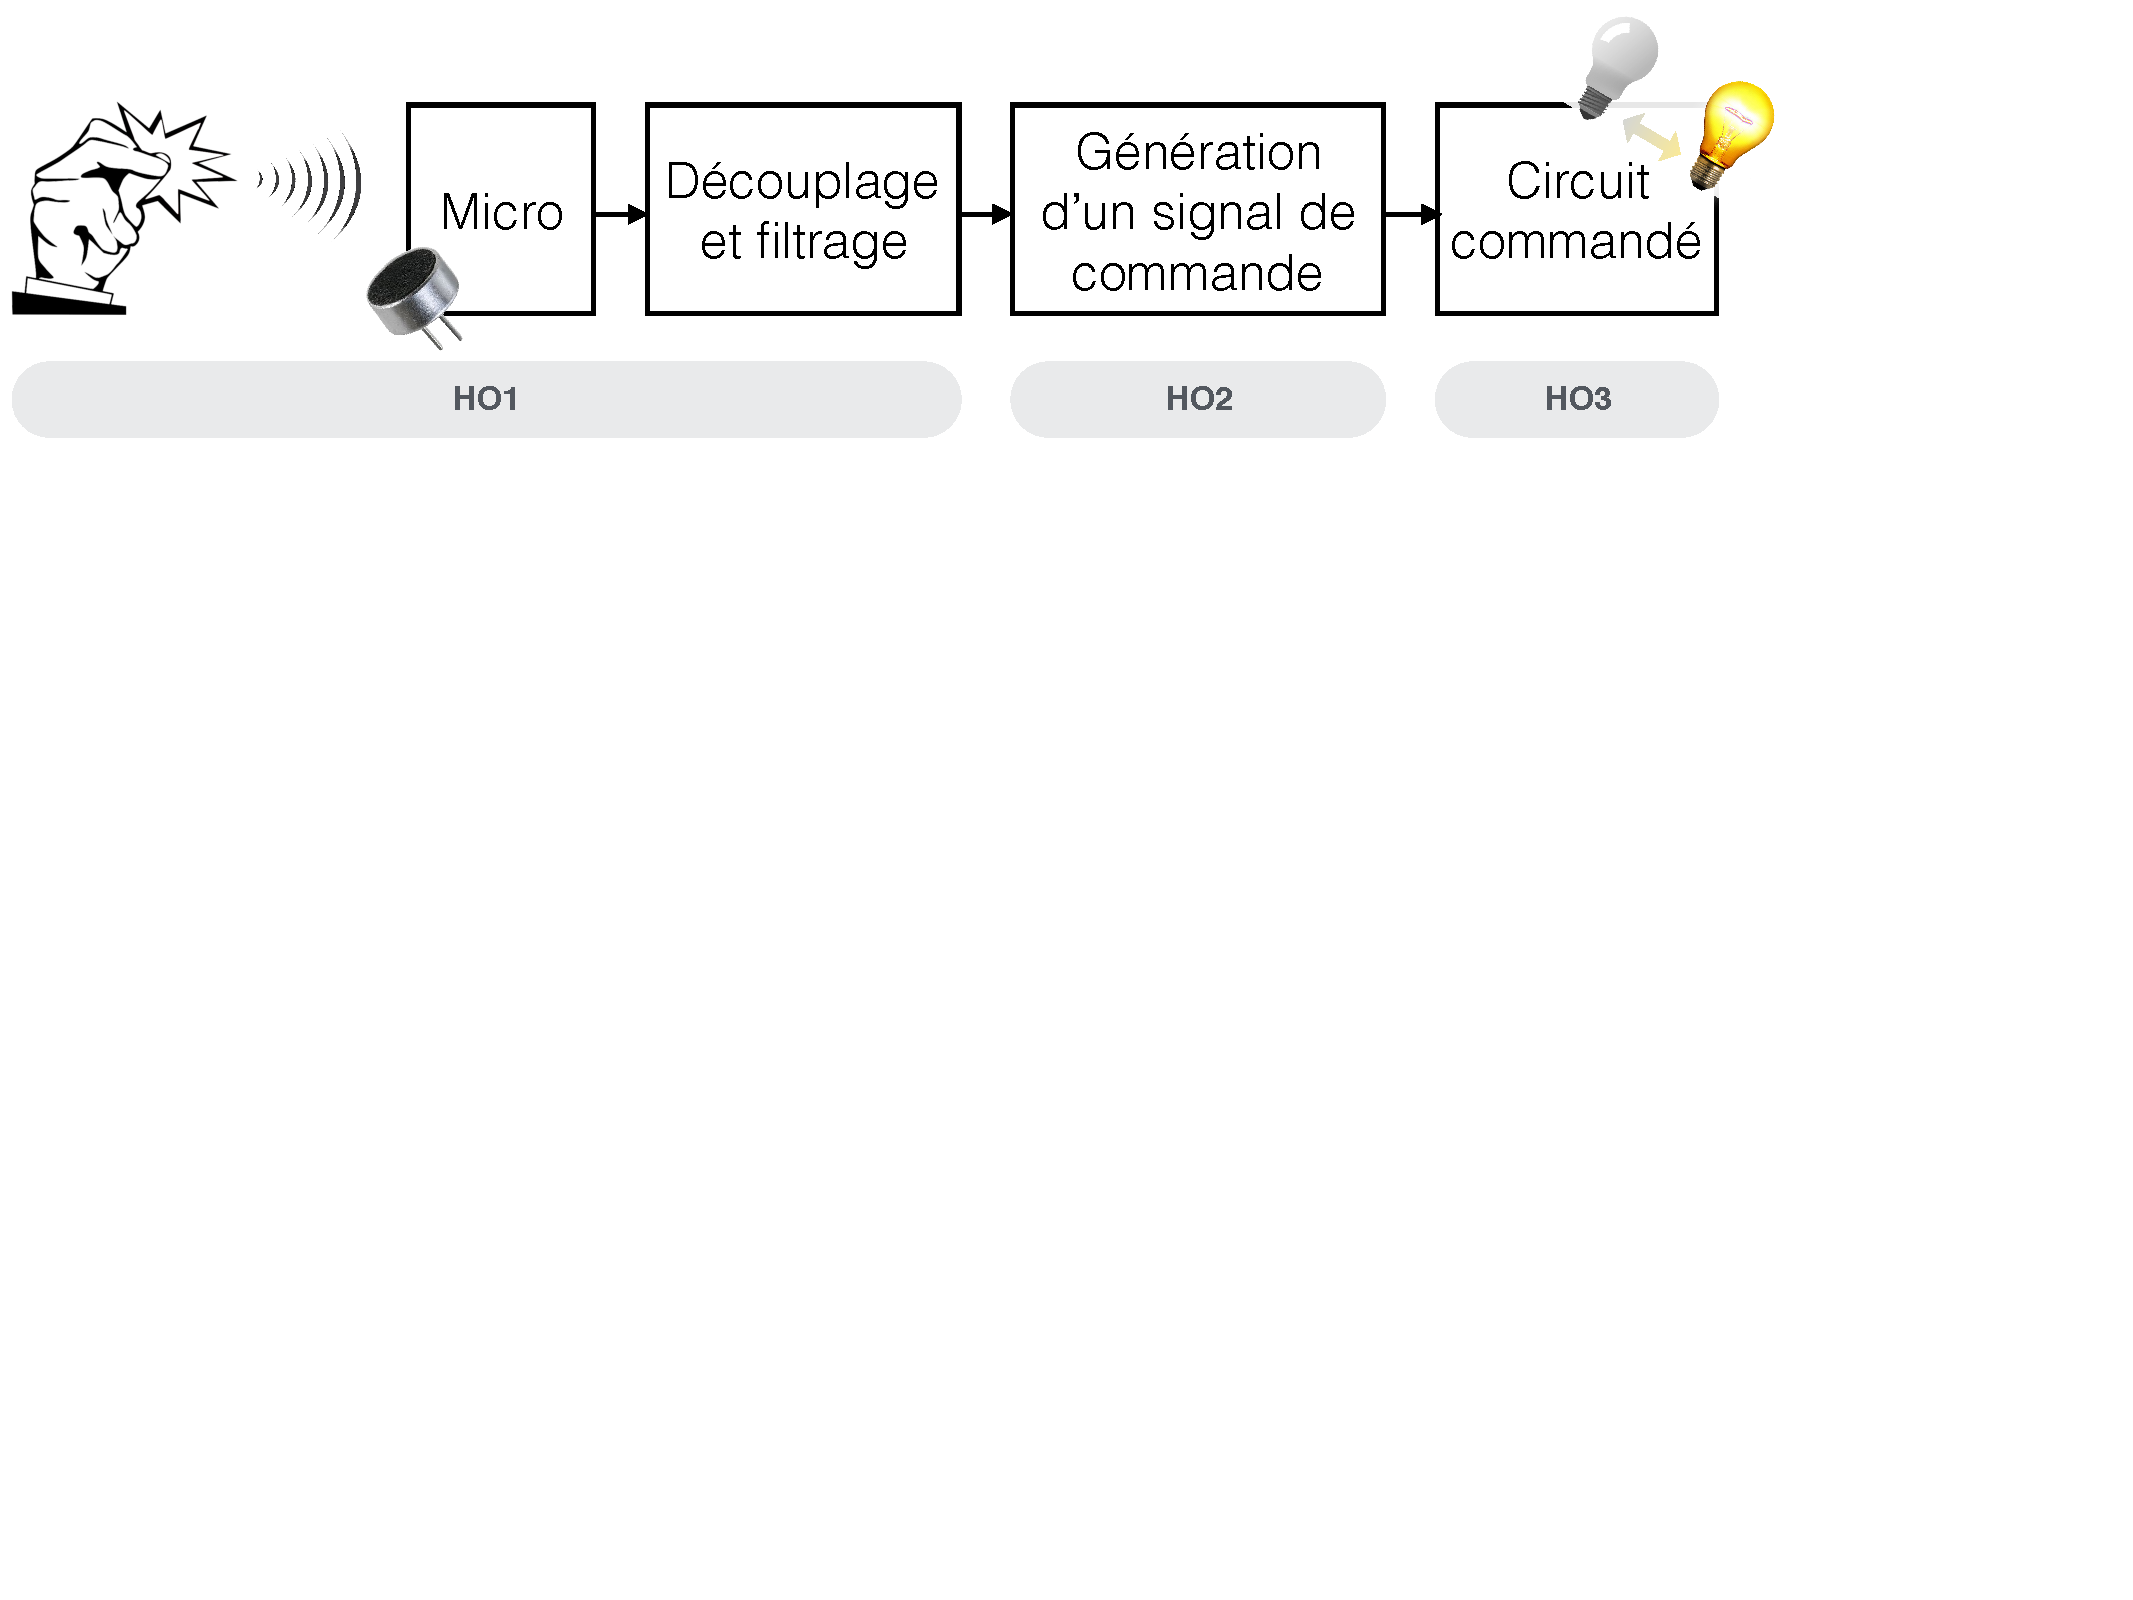
\includegraphics[width=.75\textwidth]{figures/SchemaBloc.pdf}
	\caption{Schéma-bloc du circuit.}
	\label{fig:block-diagram}
\end{figure}

Le schéma-bloc du circuit est présenté à la Figure \ref{fig:block-diagram}. Les ondes acoustiques générées par le claquement de doigt sont captées par le micro qui les transforme en un signal électrique (transduction). Ce signal est ensuite découplé et filtré à l'aide d'un filtre RC, comme présenté plus loin dans ce document. La génération d'un signal de commande propre ainsi que l'implémentation d'un circuit commandé seront abordées plus en détail dans les prochain hands-on.


\newpage

%%% Description du circuit
\section*{Description du circuit}
\begin{figure}[ht!]
	\centering
	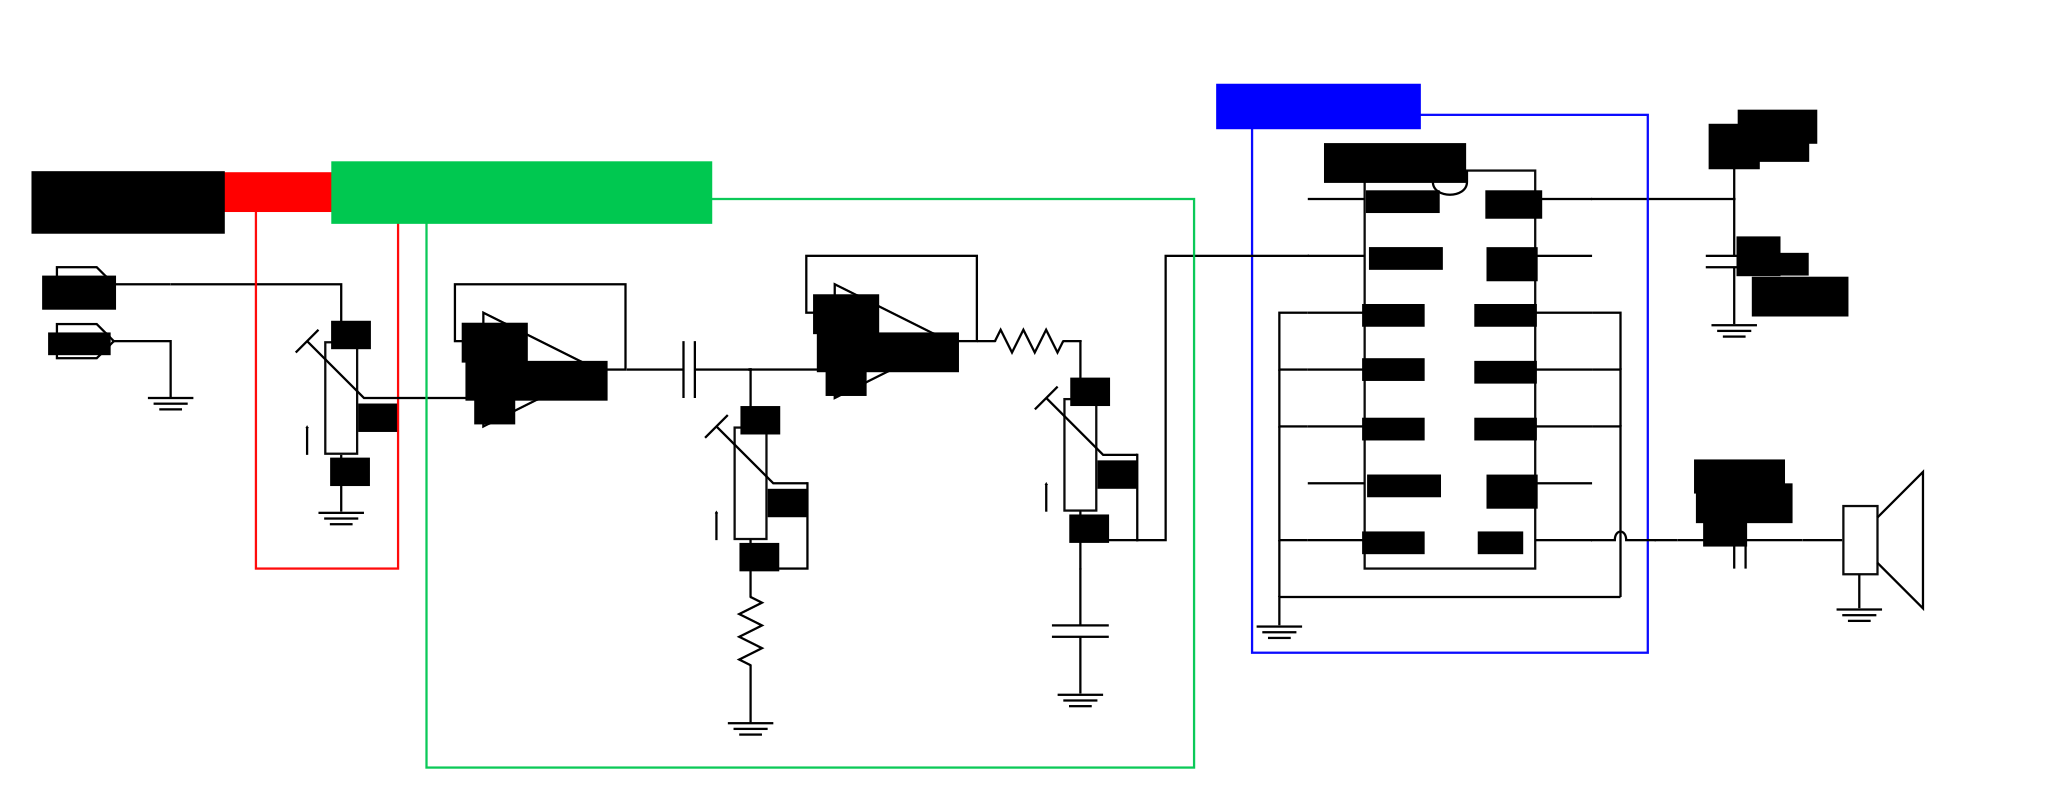
\includegraphics[width=\textwidth]{schematics}
	\caption{Schématique du circuit.}
	\label{fig2:schematics}
\end{figure}

Le schématique du circuit modifié est présenté à la Figure \ref{fig2:schematics}. En partant de la gauche, le signal d'entrée fourni par le câble jack à la borne IN1 passe d'abord dans le bloc de filtrage. Les filtres ont été implémentés sur base de topologies passe-haut et passe-bas passives, c'est-à-dire qu'elles n'utilisent pas d'amplificateur opérationnel. Pour éviter que l'impédance d'entrée (resp. sortie) des blocs suivants (resp. précédents) ait un impact sur le comportement des filtres, ceux-ci sont isolés du reste du circuit par des montages suiveurs, à savoir un amplificateur opérationnel avec une rétroaction unitaire sur la borne négative.Le signal est ensuite transmis au bloc de distorsion (de type overdrive/clipper), inspiré de la pédale appelée \textit{Dan Armstrong's Blue Clipper}. Le détail de ce circuit est présenté à la Figure \ref{fig3:clipper}. Ce bloc inclus également le contrôle du volume, implémenté par un diviseur résistif. Enfin, le signal est amplifié puis transmis au haut-parleur.

\subsection*{Diagramme de Bode}
Un diagramme de Bode est un outil pour l'analyse du comportement fréquentiel de nombreux circuits, utilisé de façon universelle par les ingénieurs électriciens.\\

Il est constitué de 2 éléments :
\begin{enumerate}
	\item Le diagramme en \textbf{amplitude} : Pour un signal sinusoïdal à une fréquence donnée, il donne le rapport d'amplitude du signal de sortie et du signal d'entrée du circuit. Ce rapport d'amplitude est généralement exprimé en décibels (dB), à savoir un rapport de puissances, dont la définition est la suivante : 
	\begin{align*}
		20 \log_{10}\left( \frac{V_{out}}{V_{in}}\right)
	\end{align*}
	\item Le diagramme en \textbf{phase} : Pour un signal sinusoïdal à une fréquence donnée, il donne le déphasage du signal de sortie par rapport au signal d'entrée, exprimé en degrés ou en radians. 
\end{enumerate}
\vspace{.25cm}

Le diagramme de Bode de la Figure \ref{fig3:lpf} donne un exemple de ce que l'on peut observer dans le cas d'un filtre passe-bas. La fréquence de coupure, représentée ici par un trait rouge, est la fréquence à partir de laquelle le filtre commence à atténuer l'amplitude du signal d'entrée. Avant cette fréquence, le signal d'entrée et de sortie ont la même amplitude. Au-delà de cette fréquence, le signal de sortie est atténué par rapport au signal d'entrée.

\begin{figure}[!ht]
	\centering
	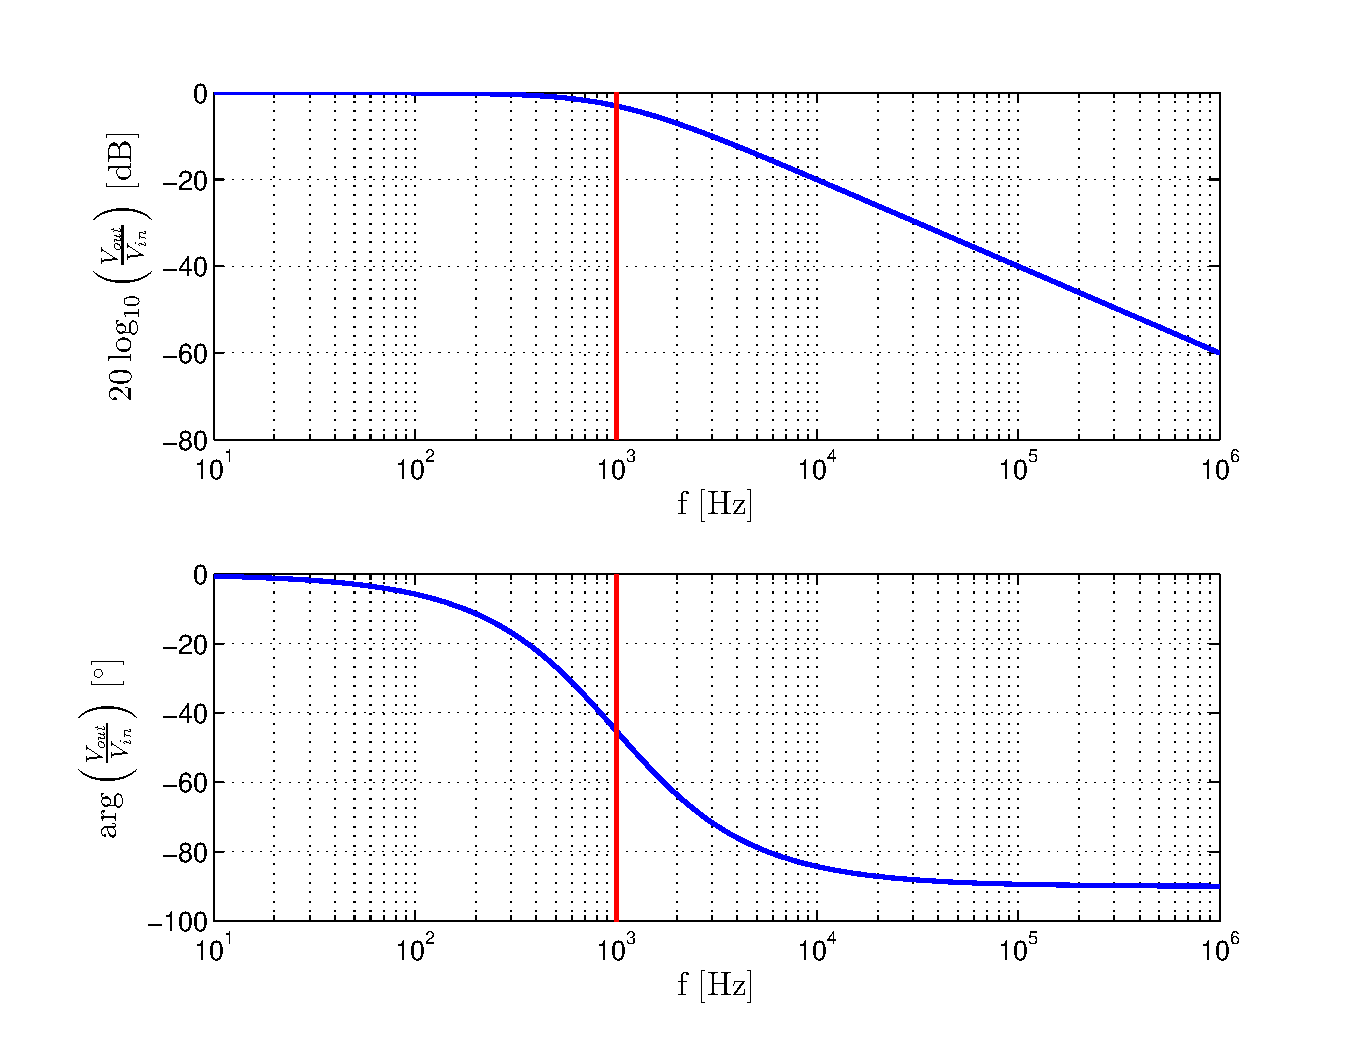
\includegraphics[width=.75\textwidth]{lpf}
	\caption{Diagramme de Bode d'un filtre passe-bas.}
	\label{fig3:lpf}
\end{figure}

\newpage

\subsection*{Montage suiveur}
% Subsection about followers

Dans le schéma de la Figure \ref{fig2:schematics}, les filtres passifs sont isolés les uns des autres grâce à des \emph{amplificateurs}, placés dans des montages suiveurs. Pour réaliser ces montages, nous allons utiliser un chip, le LM358N, représenté sur la Figure \ref{fig:LM358N_pic}, qui contient en fait deux amplificateurs. Ce chip a aussi une encoche pour donner l'information sur le sens de branchement. Chaque patte/pin du circuit a une fonction différente, comme renseigné sur la Figure \ref{fig:LM358N_pins}. Par exemple, la patte $V_{cc-}$ (pin 4) doit être connectée à une alimentation de $-15 V$ et la patte $V_{cc+}$ (pin 8) doit être connectée à une alimentation de $+15 V$. Les pins 1 à 3 sont les entrées/sortie du premier amplificateur, les pins 5 à 7 sont celles du second.

\begin{minipage}[c]{.49\textwidth}
	\centering
	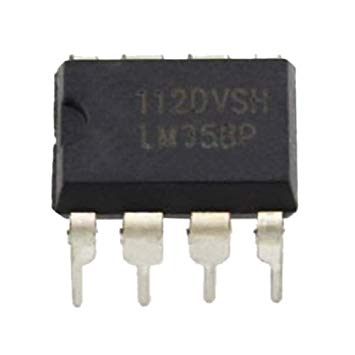
\includegraphics[width=0.6\textwidth]{figures/LM358N_picture.jpg}
	\captionof{figure}{Photo de du chip LM358N.}
	\label{fig:LM358N_pic}
\end{minipage}
\hfill
\begin{minipage}[c]{.49\textwidth}
	\centering
	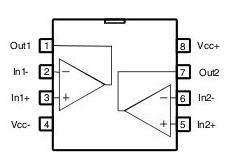
\includegraphics[width=\textwidth]{figures/LM358N_connections.jpg}
	\captionof{figure}{Nom des pattes du chip LM358N.}
	\label{fig:LM358N_pins}
\end{minipage}
\vspace{1cm}

Un \emph{montage suiveur} consiste à connecter la sortie d'un amplificateur à son entrée négative ($IN-$). La sortie va alors \emph{suivre} l'entrée positive ($IN+$). Ce montage permet d'isoler ce qui suit l'amplificateur de ce qui le précède, car l'amplificateur a une haute impédance d'entrée et une très faible impédance de sortie.

\subsection*{Filtre passe-haut}
% Subsection about HPF
Le premier filtre implémenté est un \emph{filtre passe-haut} (ou \emph{High-Pass Filter}, HPF en anglais). Il s'agit d'un filtre qui laisse passer les hautes fréquences et filtre les signaux à basse fréquence. 

Une manière simple de mettre en oeuvre ce type de filtre est d'utiliser une capacité suivie d'une résistance vers la masse (voir Figure \ref{fig2:schematics}). La capacité va laisser passer les signaux à haute fréquence. La \emph{fréquence de coupure} du filtre, c'est-à-dire la fréquence $f_c$ à partir de laquelle le filtre HPF va commencer à laisser passer le signal, est inversément proportionnelle à $RC$:
\[
	f_c = \dfrac{1}{2\pi RC}.
\]

Pour pouvoir contrôler/modifier l'effet du filtre, il suffit d'utiliser un potentiomètre (une résistance variable) à la place d'une résistance fixe.

\subsection*{Filtre passe-bas}
% Subsection about LPF
Le second filtre implémenté est un \emph{filtre passe-bas} (ou \emph{Low-Pass Filter}, LPF en anglais). Il s'agit d'un filtre qui laisse passer les basses fréquences et filtre les signaux à haute fréquence. 

De nouveau, une manière simple de mettre en oeuvre ce type de filtre est d'utiliser une résistance suivie d'une capacité vers la masse (voir Figure \ref{fig2:schematics}). La capacité va court-circuiter à la masse les signaux à haute fréquence, laissant donc passer les signaux à basse fréquence. La \emph{fréquence de coupure} du filtre, c'est-à-dire la fréquence $f_c$ à partir de laquelle le filtre LPF va commencer à couper le signal, est inversément proportionnelle à $RC$:
\[
	f_c = \dfrac{1}{2\pi RC}.
\]

Pour pouvoir contrôler/modifier l'effet du filtre, il suffit d'utiliser un potentiomètre (une résistance variable) à la place d'une résistance fixe.

\end{document}